\documentclass{article}

\usepackage{parskip}
\usepackage{titlesec}
\usepackage{hyperref}
\usepackage{xstring}
\usepackage{graphicx}

% Move the title up a bit.
\usepackage{titling}
\setlength{\droptitle}{-10ex}

% Describe how code should be syntax-highlighted.
\usepackage{minted}
\usemintedstyle{borland}

% Define aliases for python and bash minted environments.
\newminted{python}{fontsize=\small}
\newminted{bash}{fontsize=\small}

% Use the "courier" font for code listings.  Unlike the default monospace font, 
% courier can be bolded and doesn't look funny when italicized.
\usepackage{courier}

% Describe how the TOC should be formatted.
\usepackage{tocloft}
\renewcommand\cftsecleader{\cftdotfill{\cftdotsep}}
\renewcommand\cftsecfont{\normalfont}
\renewcommand\cftsecpagefont{\normalfont}
\setlength{\cftbeforesecskip}{0.0ex}

% Specify how hyperlinks should be colored.
\hypersetup{
  colorlinks = true,
  urlcolor   = blue,
  linkcolor  = black,
  citecolor  = black
}

% In description lists, start each description on it's own line.
\usepackage{enumitem}
\setlist[description]{style=nextline}

% Don't number sections, and start each section on a new page.
\setcounter{secnumdepth}{0}
\newcommand{\sectionbreak}{\clearpage}

% Define commands for managing the TOC.
\makeatletter
\newcommand\organizedtoc{%
    \subsubsection*{Making the code available}\@starttoc{use}%
    \subsubsection*{Documenting the code}\@starttoc{doc}%
    \subsubsection*{Testing the code}\@starttoc{test}}
\newcommand\organizedsection[2]{
 \section{#2}
 \addcontentsline{#1}{section}{#2}
 \setcounter{footnote}{1}}
\makeatother

% Define a command to typeset links in a way that's readable in print.
\usepackage{xifthen}
\newcommand{\link}[2]{#1\footnote{\url{#2}}}
\renewcommand*{\thefootnote}{\fnsymbol{footnote}}

% Define a command for typesetting module names.  A URL can optionally be 
% given, in which case it will be added as a footnote and a hyperlink.
\usepackage{xifthen}
\newcommand{\module}[2][]{%
 \ifthenelse{\isempty{#1}}%
 {\texttt{#2}}%
 {\link{\texttt{#2}}{#1}}%
}

% Define a command to include files from the kbkdna module.
\newcommand{\kbkdnafile}[2]{%
\begin{listing}[h]%
 \inputminted[fontsize=\small]{#1}{../kbkdna/#2}%
 \caption{\texttt{\detokenize{#2}}}%
\end{listing}}

\begin{document}

\title{How to publish python code}
\author{Kale Kundert}
\date{2016 Kortemme Lab Retreat}
\maketitle{}

Once you get some code to work, it's easy to not bother making that code easy 
for other people to use.  Usually you have more pressing things to worry about, 
and it's hard to even know what you could do to help other people use your code 
anyway.  However, especially as scientists, we have a responsibility to make 
the code we write easily accessible to anyone who wants or needs to use it.

In this tutorial, we'll walk through all the steps required to publish some 
python code.  The example code we'll be working with will manipulate DNA 
sequences in simple ways.  Specifically, it'll calculate lengths, GC contents, 
and reverse complements.  We'll expose this functionality both as a library and 
as a command-line tool.

Broadly speaking, there are three things we need to do to publish code.  These 
are making the code available, documenting the code, and testing the code.  
Each of these larger objectives can be broken down into a handful of very 
concrete steps which this tutorial will describe:

\organizedtoc

\organizedsection{use}{Organizing your files}

Most python projects organize their files in the same way.  This standard 
directory layout is pretty simple and works well in every situation I've ever 
encountered.  By adhering to it, you make your code easier for others to grok 
and you avoid getting tied into knots by bad organizational decisions.

The first step is to choose a name for your project.  This name has to be 
unique (i.e. there can't be any other python packages with the same name) and 
it should somehow reflect what your code actually does.  The name I'll use for 
this tutorial is \module{kbkdna}, because my initials are \texttt{kbk} and the 
code will deal with DNA.  You should use your own initials instead, because you 
won't be able to publish a package with the same name as mine.

\begin{listing}[h]
\begin{bashcode}
# Make a directory for the project and move into it.
$ mkdir kbkdna
$ cd kbkdna

# Make a README file.
$ touch README.rst

# Make a LICENSE file.
$ touch LICENSE.txt

# Make a directory for your python code.
$ mkdir kbkdna
$ touch kbkdna/__init__.py

# Make a directory for your documentation.
$ mkdir docs

# Make a directory for your tests.
$ mkdir tests

# Make sure everything was created properly.
$ ls
docs/  kbkdna/  tests/  README.rst  LICENSE.txt

\end{bashcode}
\end{listing}

\organizedsection{use}{Hosting your code on Github}

Version control is useful for many reasons, but two in particular are worth 
mentioning here.  First, it allows you to go back to old versions of your code 
if you have to, which allows you to tinker with working code more fearlessly.  
Second, it makes it easy to share your code with other people and for other 
people to contribute to your project.  This is especially true if you host your 
repository on a popular site like \link{GitHub}{https://github.com/}.

The first step is to turn your project directory into a git repository and to 
commit all the files you've made so far:

\begin{bashcode}
$ git init
$ git commit -a -m "Initial commit"
\end{bashcode}

Next, log into GitHub.  You'll have to create an account if you don't already 
have one.  Then find the ``New repository'' button and click it.  Give the 
repository the same name as your project and provide a brief description for 
it.  The defaults are fine for the rest of the options.

\begin{figure}[h]
 \frame{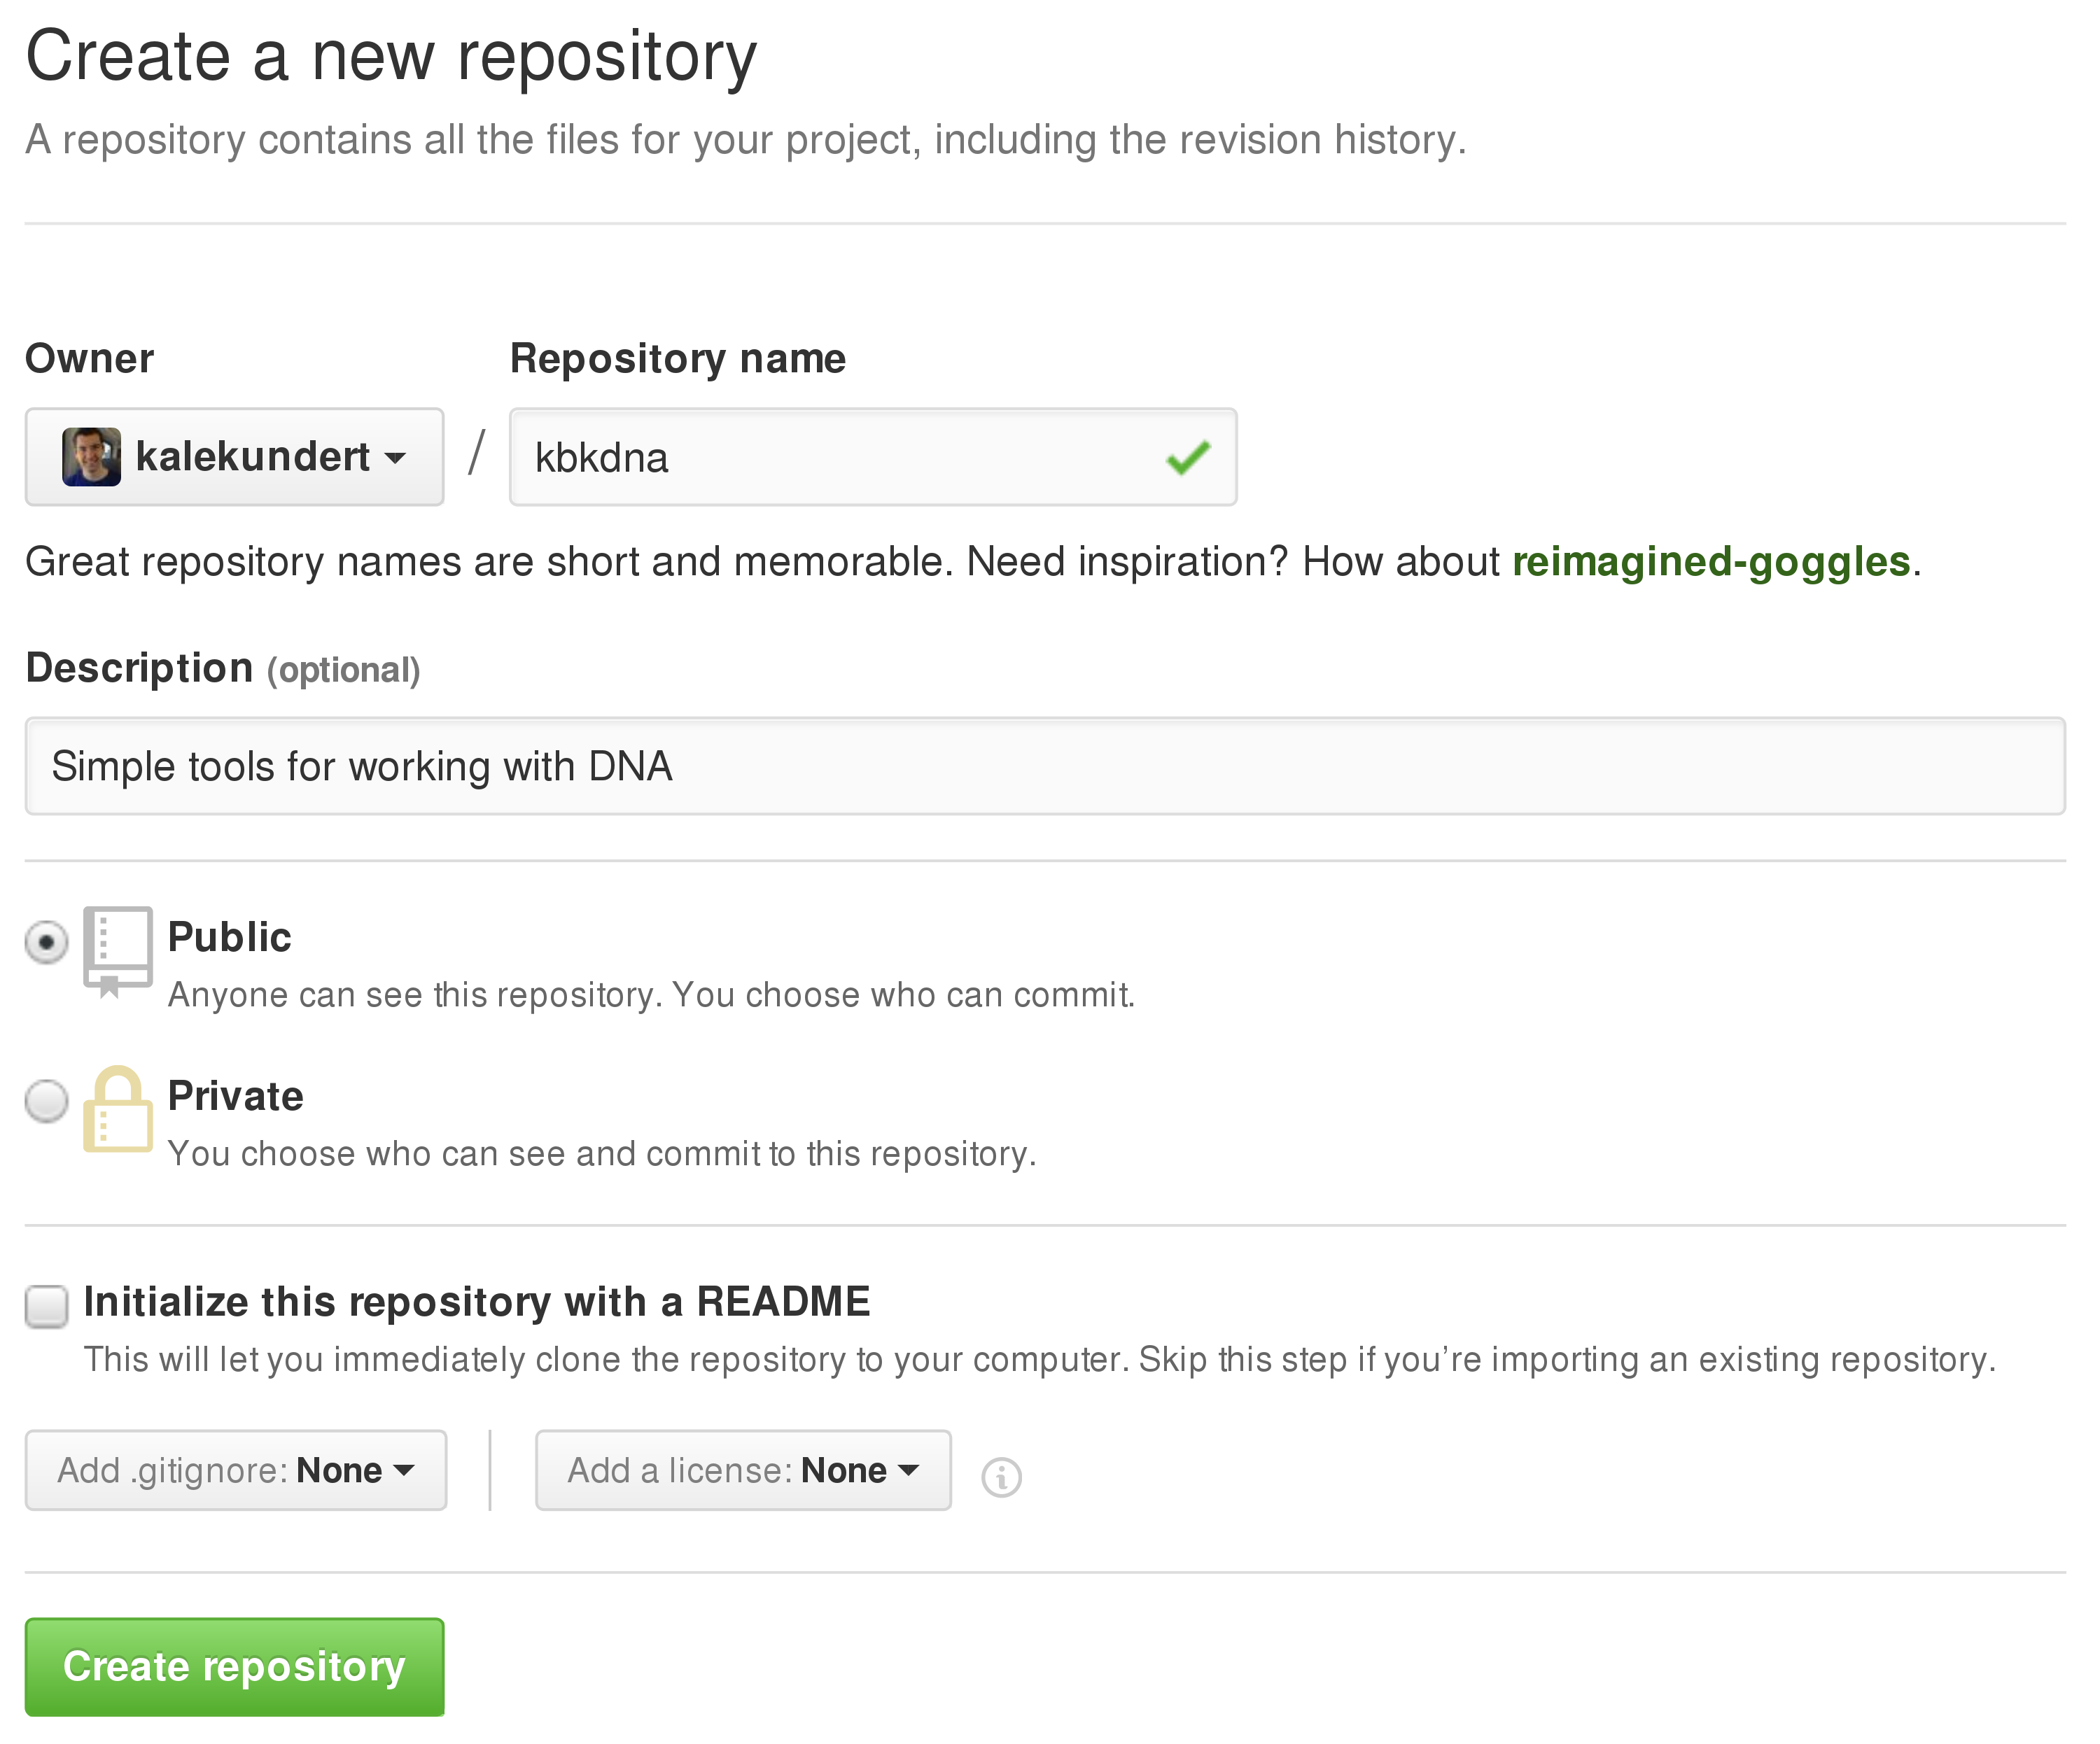
\includegraphics[width=\textwidth]{screenshots/github}}
\end{figure}

The next page will tell you the commands you need to run to connect the 
repository you made for your project with \texttt{git init} with this new one 
being hosted by GitHub.  Here are the commands I ran:

\begin{bashcode}
$ git remote add origin git@github.com:kalekundert/kbkdna.git
$ git push -u origin master
\end{bashcode}

\organizedsection{misc}{Writing some example functions}

Below are the four functions making up the library we want to publish.  Nothing 
about this code is particular to how we will publish it; it's just regular 
python code.  Copy it into \texttt{kbkdna/dna.py}:

\kbkdnafile{python}{kbkdna/dna.py}

Also add the following code to \texttt{kbk/\_\_init\_\_.py}:

\kbkdnafile{python}{kbkdna/__init__.py}

\organizedsection{doc}{Providing command-line help with \module{docopt}}

Along with our library, we want to provide a program to manipulate DNA 
sequences from the command-line.  This program will read a sequence and a 
desired manipulation (i.e. length, GC content, reverse complement) from the 
command line, and will print out the result of that manipulation.  Documenting 
the arguments that this program expects is a crucial part of making this 
program usable for other people.  This should be done in two ways:

\begin{enumerate}
 \item If the program receives arguments that don't make sense, it should print 
  a brief usage hint.
 \item If the user provides the \texttt{-h} or \texttt{--help} flag, the 
  program should print a detailed help message.  This message should include a 
  few sentences saying what the program is supposed to do and a description of 
  every single argument the program takes.
\end{enumerate}

There are several ways to do both these things in python, but the 
\module[http://docopt.org/]{docopt} module is by far my favorite.  We just need 
to write a help message at the top of our script describing the arguments we 
expect.  \module{docopt} will read that message and use it to parse the 
command-line arguments for us.  If there are any problems, it will print a 
usage hint and end the program.  If not, it will give us a dictionary 
containing the parsed arguments.

The thing I love about \texttt{docopt} is that it combines a good help message, 
which is good for users, with easy command-line argument parsing, which is good 
for me.  I've found that I'm much more likely to write documentation when 
there's an immediate benefit in it for me!

There's an example on the following page.  Copy it into \texttt{kbkdna/cli.py}.  
There are parts of this code that are particular to how we will publish it, 
specifically the relative import and the main function that's never called, so 
don't bother trying to run it yet.

\kbkdnafile{python}{kbkdna/cli.py}

\organizedsection{use}{Writing a \texttt{setup.py} file}

The best way to install python software that other people have written is to 
use a tool called \module[https://packaging.python.org/installing/]{pip}.  You 
just need to give the name of the software you want to install.  For example, 
here is the command to install \module{docopt}:

\begin{bashcode}
 $ pip install docopt
\end{bashcode}

To make this work for our project, we need to specify some additional 
information in a file called \texttt{setup.py}.

\kbkdnafile{python}{setup.py}

The \texttt{name} field is the name that other people will eventually use to 
refer to our project.  The \texttt{packages} field is a list of directories 
containing the python code to install.  The \texttt{install\_requires} field is 
a list of other packages that our project makes use of.  Whenever our project 
is installed, these will automatically be installed as well.  The 
\texttt{entry\_points} field is confusing, but it says we want to create a 
command-line application called \texttt{dna} to run our \texttt{main()} 
function.  The rest of the fields are optional metadata and are hopefully 
pretty self-explanatory.

We can now use \module{pip} to install our project for ourselves:

\begin{bashcode}
 $ pip install -e .
\end{bashcode}

The \texttt{-e} flag tells \module{pip} to install your code in \emph{editable} 
mode, so that any changes we make are automatically applied without us having 
to rerun the \texttt{install} command.

The advantage of using writing a \texttt{setup.py} file and using \module{pip} 
to install your code is that it is now available anywhere on your computer.  No 
matter what directory you're in, you can import and run your code.  This may 
seem like a small thing, but it can make organizing your scripts dramatically 
easier.  It can also encourage you to make a set of general-purpose utility 
functions, which can save you time if you tend to write similar functions in 
many different projects.

\organizedsection{use}{Uploading your package to PyPI}

In order for other people to be able to install our software using 
\module{pip}, we need to upload it to the \link{Python Package Index 
(PyPI)}{https://pypi.python.org/pypi}, a global repository of python software 
that anyone can contribute to.  The first step is to register an account on 
PyPI:

\begin{figure}[h]
 \frame{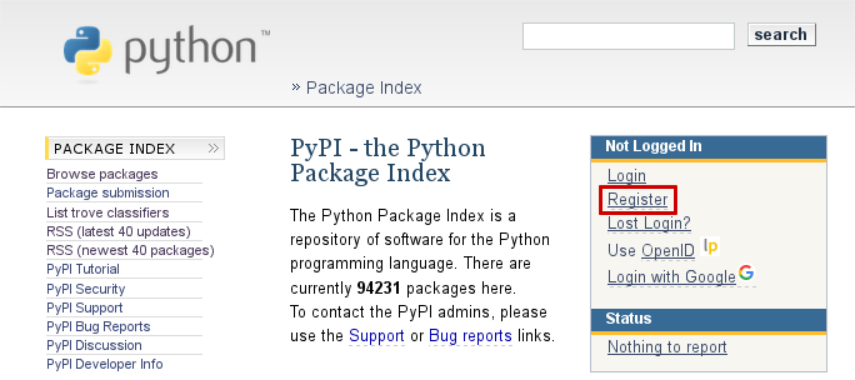
\includegraphics[width=\textwidth]{screenshots/pypi}}
 \caption{\url{https://pypi.python.org/pypi}}
\end{figure}

Once you've done that, run the following two commands to register and upload 
your project.  You only need to run the \texttt{register} command one time for 
each project.  You can run the \texttt{sdist upload} command whenever you want 
to upload a new version of your project, but you will need to increment the 
version number in \texttt{setup.py} each time.

\begin{bashcode}
 $ python setup.py register
 $ python setup.py sdist upload
\end{bashcode}

Now anyone should be able to install your code the same way they would install 
any other code:

\begin{bashcode}
 $ pip install kbkdna
\end{bashcode}

\organizedsection{doc}{Writing a \texttt{README.rst} file}

A \texttt{README} file should briefly explain what the project is supposed to 
do, how to install it, and how to use it.  I also like to include a few 
``badges'' to advertise that the project can be installed using the standard 
tools, that it passes its tests, and that its documentation is available online 
(which are all things we'll get to in this tutorial).

The \texttt{*.rst} suffix means that the file is reStructuredText.  This is a 
simple file format is supposed to look good as raw text while still being easy 
to convert to HTML.  The two important things to know are that you can start a 
new section by underlining the title of that section with equal signs or 
dashes, and you enter a block of code by ending the previous paragraph with two 
colons and indenting the code block.

\kbkdnafile{text}{README.rst}

\organizedsection{use}{Choosing a license}

Choosing a license is important because it lets other people know how they can 
use your code.  The website \url{choosealicense.com} is a good resource where 
you can compare a number common licenses and find one you like.  The two most 
common choices for academic code are the MIT license and the GPLv3 license:

\begin{description}
\item[MIT License] No restrictions on how your code can be used.  This allows 
 your code to be included with commercial software.
\item[GPLv3 License] Requires that any derivatives of your code be made 
 publicly available.  This effectively forbids your code from being included 
 with commercial software.
\end{description}

I'll use the MIT license for \module{kbkdna} because it's short enough to fit 
on one page.

\kbkdnafile{text}{LICENSE.txt}

\organizedsection{doc}{Writing documentation with Sphinx}

Sphinx is a tool that 

\begin{bashcode}
 $ pip install sphinx
 $ sphinx-quickstart docs
\end{bashcode}

\organizedsection{doc}{Uploading documentation to ReadTheDocs}

\organizedsection{test}{Writing tests with \module{pytest}}

Published code should be tested, both to convince yourself and to convince your
users that the code works.  There are many ways to test your code, but 
\module[http://doc.pytest.org/en/latest/]{pytest} is my favorite because it 
requires very little boilerplate, produces clear output, and integrates nicely 
with the debugger.  Here are what some tests for our project might look like.  
Copy this file into \texttt{tests/test\_dna.py}:

\kbkdnafile{python}{tests/test_dna.py}

\module{pytest} will look for tests in files whose name begins with 
\texttt{test\_}.  Within those files, each test is just a normal function whose 
name also begins with \texttt{test\_}.  Within those functions, use python's 
\mintinline{python}|assert| statement to test your code.

Install and run \module{pytest} using the following commands:

\begin{bashcode}
 $ pip install pytest
 $ py.test
\end{bashcode}

This should print a big red error message, explaining that the GC content of 
\texttt{ATGC} was expected to be 50\%, but was incorrectly calculated to be 
0\%.  This bug is due to integer division in the 
\mintinline{python}|gc_content()| function, and we can fix it by adding the 
following line\footnote{It's a good idea to put this line in all of your 
\texttt{python2} scripts.} right after the shebang line in 
\texttt{kbkdna/dna.py}:

\begin{pythoncode}
 from __future__ import division
\end{pythoncode}

If you run the tests again, they should pass and you should get a nice green 
success message.

\organizedsection{test}{Running tests on TravisCI}

\organizedsection{misc}{Using \module{cookiecutter}}

\end{document}

